\documentclass[11pt,a4paper]{article}
\usepackage[margin=25mm]{geometry}
\usepackage[T1]{fontenc}
\usepackage[utf8]{inputenc}
\usepackage{lmodern}
\usepackage{microtype}
\usepackage{amsmath,amssymb,mathtools,bm}
\usepackage{booktabs,tabularx,longtable,array,multirow}
\usepackage{graphicx,subcaption,float,placeins}
\usepackage[dvipsnames]{xcolor}
\usepackage{tikz}
\usepackage{pdflscape}
\usetikzlibrary{arrows.meta,positioning,fit,calc,backgrounds}
\usepackage{hyperref}
\usepackage{cleveref}
\usepackage{enumitem}
\usepackage{siunitx}
\usepackage{fancyhdr}
\usepackage{titlesec}
\usepackage[most]{tcolorbox}
\usepackage[numbers,sort&compress]{natbib}

\definecolor{reportblue}{HTML}{174A7E}
\definecolor{reportorange}{HTML}{D97706}
\definecolor{reportgreen}{HTML}{2E7D32}
\definecolor{reportgray}{HTML}{F4F6F8}
\hypersetup{colorlinks=true,linkcolor=reportblue,citecolor=reportblue,urlcolor=reportblue,pdftitle={Ball World Model Rotation-Only Report}}
\titleformat{\section}{\Large\bfseries\color{reportblue}}{\thesection}{0.6em}{}
\titleformat{\subsection}{\large\bfseries\color{reportblue}}{\thesubsection}{0.6em}{}
\setlength{\parindent}{0pt}
\setlength{\parskip}{0.55em}
\pagestyle{fancy}
\fancyhf{}
\lhead{Ball World Model: Rotation-Only Observer}
\rhead{14 September 2026}
\cfoot{\thepage}
\newcommand{\R}{\mathbb R}
\newcommand{\SO}{\mathrm{SO}}
\newcommand{\Exp}{\operatorname{Exp}}
\newcommand{\sg}{\operatorname{sg}}
\newcommand{\vect}[1]{\mathbf{#1}}
\newtcolorbox{keyresult}[1][]{colback=green!4,colframe=reportgreen,title=Key result,fonttitle=\bfseries,#1}
\newtcolorbox{interpretation}[1][]{colback=blue!3,colframe=reportblue,title=Interpretation,fonttitle=\bfseries,#1}
\newtcolorbox{caution}[1][]{colback=orange!4,colframe=reportorange,title=Important qualification,fonttitle=\bfseries,#1}

\begin{document}
\begin{titlepage}
\centering
\vspace*{22mm}
{\Huge\bfseries\color{reportblue} Ball World Model\par}
\vspace{5mm}
{\LARGE Architecture, Training Objectives, Representation Analysis, and Rotation-Only Evaluation\par}
\vspace{18mm}
\begin{tcolorbox}[width=.86\textwidth,colback=reportgray,colframe=reportblue,boxrule=.8pt]
\centering\large
\textbf{Core idea}\par\medskip
RGB sequence $\rightarrow$ spatial content and directed motion $\rightarrow$ orientation and angular velocity on $\SO(3)$
\end{tcolorbox}
\vfill
{\Large Dr. Jasper Juchem\par}
\vspace{4mm}
{\large A stand-alone technical reference for machine-learning and dynamical-systems researchers\par}
\vspace{12mm}
{\large Based on the rotation-only evaluation dated 14 September 2026\par}
{\large Version 1.0 - 14 September 2026\par}
\end{titlepage}

\begin{abstract}
This report documents and evaluates a visual neural observer for the rotation-only motion of a textured sphere. The sphere centre is fixed, translational velocity is zero, and the network receives ten rendered RGB frames from which it estimates an orientation matrix and world-frame angular velocity. The architecture separates configuration-like content from tangent-like motion: a coordinate-aware convolutional encoder produces spatial feature maps and compact content embeddings, while a bidirectional spatial motion encoder processes adjacent feature maps and their normalised temporal rate. Orientation is decoded from content; angular velocity is decoded from endpoint content and motion. A joint-embedding transition predicts adjacent content embeddings in both temporal directions, and an optional shared corrector refines the state using an $\SO(3)$ kinematic residual.

The evaluated checkpoint achieves a mean geodesic orientation error of \SI{0.507}{\degree}, a median error of \SI{0.468}{\degree}, and a 95th percentile of \SI{0.970}{\degree}. Angular-velocity $R^2$ exceeds 0.998 on every component. Reversing the image sequence reverses the inferred angular velocity with an average residual of \SI{0.816}{\radian\per\second}; replacing the sequence by a repeated frame reduces the inferred angular speed from \SI{29.32}{\radian\per\second} to \SI{0.382}{\radian\per\second}. Linear probes reveal a sharp representation split: the final content embedding predicts orientation with \SI{1.266}{\degree} mean error but has no useful linear angular-velocity information, whereas the learned forward and backward motion embeddings explain approximately 99.5\% of angular-velocity variance. The results support the intended content-motion factorisation and show that the observer uses temporal direction rather than static appearance shortcuts.
\end{abstract}

\tableofcontents
\clearpage

\section{Scope, provenance, and terminology}
The empirical source is the supplied evaluation archive \texttt{evaluation\_rotation\_260914.zip.txt}. The reference for report structure and level of detail is the supplied translation-only report \texttt{main.pdf}. Numerical claims in this report are calculated from the evaluation CSV and JSON files. The report is self-contained: no knowledge of the translation experiment is required.

Throughout, $B$ is batch size, $T=10$ is the number of context frames, $H=W=256$, $C=128$ is the final spatial feature count, $K=8$ is the number of soft keypoints, $D_z=256$ is content dimension, and $D_m=256$ is motion dimension. A hat denotes a prediction. The ground-truth orientation is $R_t^{\mathrm{gt}}\in\SO(3)$ and the world-frame angular velocity is $\omega_t^{\mathrm{gt}}\in\R^3$.

\begin{interpretation}
The network is best classified as a \textbf{finite-window visual state observer with a one-step joint-embedding transition}. It estimates current rotational state from observed images. It is not yet an autonomous long-horizon world model because the motion embedding for interval $t$ is computed from both observed endpoint feature maps.
\end{interpretation}

\section{Problem formulation}
\subsection{Controlled rotation-only experiment}
The ball is held at a fixed world position and has zero linear velocity. Gravity, drag, and contact effects are absent. Initial orientation and angular velocity vary across trajectories, while sphere radius, marker layout, material parameters, rendering, and camera remain fixed. This design isolates rotational observability from translation, impact, and changing appearance scale.

The network input is
\begin{equation}
\vect I_{1:T}\in\R^{B\times T\times 3\times256\times256},\qquad T=10.
\end{equation}
The supervised targets are
\begin{equation}
R_{1:T}^{\mathrm{gt}}\in\SO(3)^{B\times T},\qquad
\vect\omega_{1:T}^{\mathrm{gt}}\in\R^{B\times T\times3}.
\end{equation}
The simulator labels are not inputs to the neural forward pass. At inference,
\begin{equation}
\vect I_{1:T}\longmapsto (\hat R_{1:T},\hat{\vect\omega}_{1:T}).
\end{equation}

At \SI{100}{Hz}, $\Delta t=\SI{0.01}{s}$ and a ten-frame context spans nine intervals, or \SI{0.09}{s}. At an angular speed near the evaluated mean of \SI{29.3}{\radian\per\second}, a typical context covers roughly \SI{151}{\degree} of net angular travel. The marker pattern therefore changes substantially across a window even though the ball centre remains fixed.

\subsection{Why orientation differs from position}
Position belongs to Euclidean space. Orientation belongs to the nonlinear manifold $\SO(3)$. A valid prediction must satisfy
\begin{equation}
R^\mathsf T R=I,\qquad \det R=1.
\end{equation}
Euler angles are discontinuous and coordinate dependent; quaternions have a double-cover ambiguity. The observer therefore predicts a continuous 6D representation and projects it to $\SO(3)$ using Gram--Schmidt orthogonalisation, following a standard neural rotation representation pattern \citep{zhou2019rotation6d}.

\section{End-to-end architecture}
\begin{figure}[H]
\centering
\resizebox{\textwidth}{!}{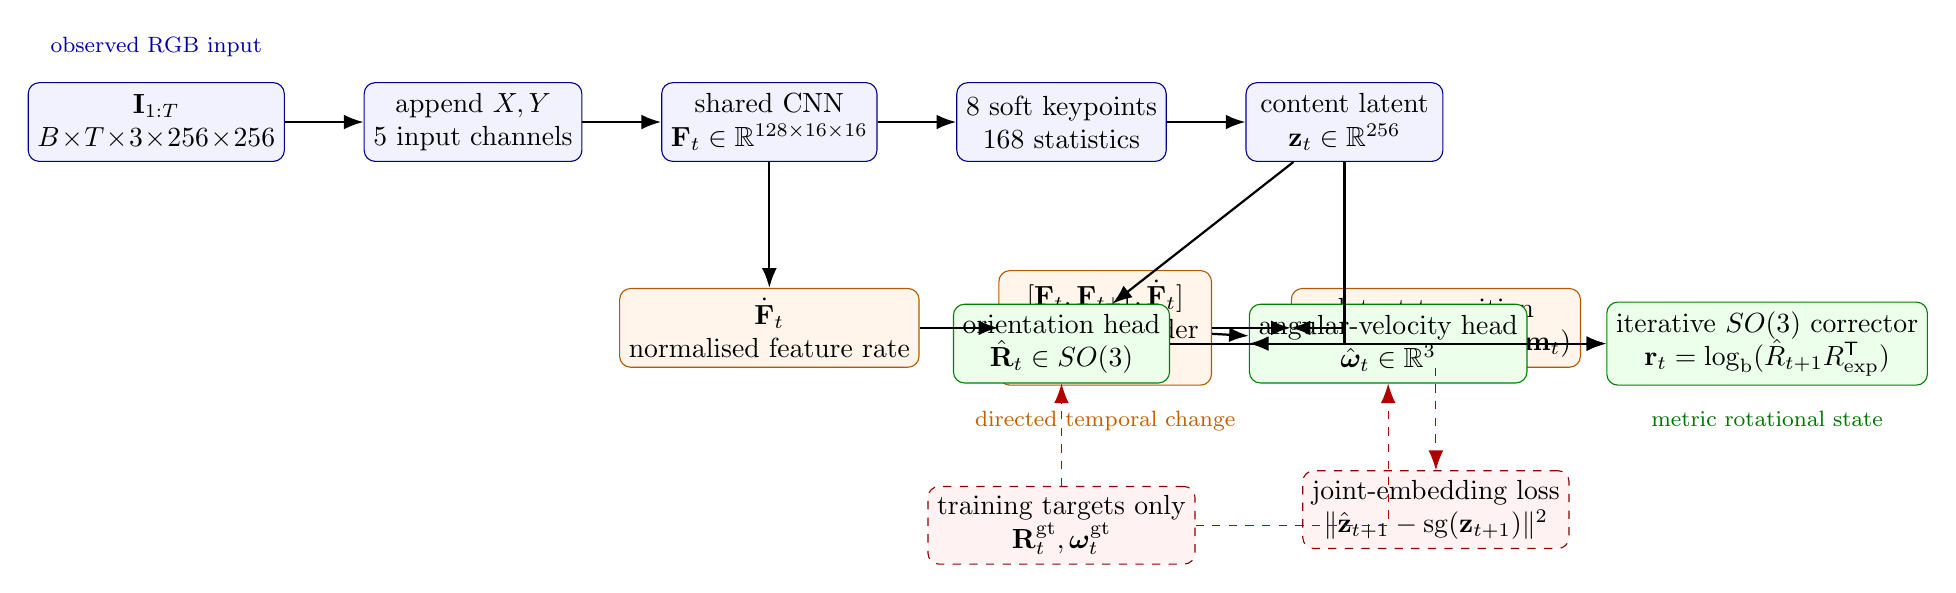
\begin{tikzpicture}[
  node distance=8mm and 10mm,
  block/.style={draw=blue!55!black, fill=blue!5, rounded corners, align=center, minimum height=10mm, minimum width=25mm},
  motion/.style={draw=orange!70!black, fill=orange!8, rounded corners, align=center, minimum height=10mm, minimum width=27mm},
  state/.style={draw=green!50!black, fill=green!8, rounded corners, align=center, minimum height=10mm, minimum width=25mm},
  loss/.style={draw=red!55!black, fill=red!5, rounded corners, dashed, align=center, minimum height=9mm},
  arrow/.style={-{Latex[length=2.5mm]}, thick},
  target/.style={-{Latex[length=2.5mm]}, dashed, red!70!black}
]
\node[block] (images) {$\mathbf I_{1:T}$\\$B\!\times\!T\!\times\!3\!\times\!256\!\times\!256$};
\node[block, right=of images] (coord) {append $X,Y$\\5 input channels};
\node[block, right=of coord] (cnn) {shared CNN\\$\mathbf F_t\in\mathbb R^{128\times16\times16}$};
\node[block, right=of cnn] (key) {8 soft keypoints\\168 statistics};
\node[block, right=of key] (content) {content latent\\$\mathbf z_t\in\mathbb R^{256}$};

\node[motion, below=16mm of cnn] (diff) {$\dot{\mathbf F}_t$\\normalised feature rate};
\node[motion, right=of diff] (motion) {$[\mathbf F_t,\mathbf F_{t+1},\dot{\mathbf F}_t]$\\motion encoder\\$\mathbf m_t\in\mathbb R^{256}$};
\node[motion, right=of motion] (transition) {latent transition\\$\hat{\mathbf z}_{t+1}=\mathbf z_t+\Delta t\,T_\theta(\mathbf m_t)$};

\node[state, below=18mm of key] (rot) {orientation head\\$\hat{\mathbf R}_t\in SO(3)$};
\node[state, right=of rot] (omega) {angular-velocity head\\$\hat{\boldsymbol\omega}_t\in\mathbb R^3$};
\node[state, right=of omega] (correct) {iterative $SO(3)$ corrector\\$\mathbf r_t=\log_{\rm b}(\hat R_{t+1}R_{\rm exp}^{\mathsf T})$};

\node[loss, below=13mm of rot] (labels) {training targets only\\$\mathbf R_t^{\rm gt},\boldsymbol\omega_t^{\rm gt}$};
\node[loss, below=13mm of transition] (latentloss) {joint-embedding loss\\$\|\hat{\mathbf z}_{t+1}-\operatorname{sg}(\mathbf z_{t+1})\|^2$};

\draw[arrow] (images)--(coord);
\draw[arrow] (coord)--(cnn);
\draw[arrow] (cnn)--(key);
\draw[arrow] (key)--(content);
\draw[arrow] (cnn)--(diff);
\draw[arrow] (diff)--(motion);
\draw[arrow] (motion)--(transition);
\draw[arrow] (content)|-(transition);
\draw[arrow] (content)--(rot);
\draw[arrow] (content)|-(omega);
\draw[arrow] (motion)--(omega);
\draw[arrow] (rot)--(correct);
\draw[arrow] (omega)--(correct);
\draw[target] (labels)--(rot);
\draw[target] (labels)-|(omega);
\draw[target] (transition)--(latentloss);

\node[font=\footnotesize, blue!65!black, above=2mm of images] {observed RGB input};
\node[font=\footnotesize, orange!75!black, below=2mm of motion] {directed temporal change};
\node[font=\footnotesize, green!45!black, below=2mm of correct] {metric rotational state};
\end{tikzpicture}
}
\caption{Rotation-only computation graph. Solid arrows are inference paths; dashed arrows denote learning targets and consistency constraints.}
\label{fig:architecture}
\end{figure}

The architecture preserves the same content-motion hypothesis that succeeded for translation:
\begin{align}
\vect F_t &= E_F(\vect I_t),\\
\vect z_t &= E_z(\vect F_t),\\
\vect m_t^+ &= E_m(\vect F_t,\vect F_{t+1},\operatorname{norm}(\dot{\vect F}_t)),\\
\hat R_t &= h_R(\vect z_t),\\
\hat{\vect\omega}_t^+ &= h_\omega(\vect z_t,\vect z_{t+1},\vect m_t^+).
\end{align}
Absolute orientation is decoded from content. Angular velocity is decoded from directed visual change while retaining endpoint content, because an identical local marker displacement can have different interpretation under different orientations and viewing geometry.

\section{Coordinate-aware frame encoder}
\subsection{Coordinate augmentation}
Two deterministic coordinate planes are appended to RGB. For pixel indices $(i,j)$,
\begin{equation}
X_{ij}=2\frac{j}{W-1}-1,\qquad Y_{ij}=2\frac{i}{H-1}-1.
\end{equation}
Thus the encoder receives five channels. Explicit coordinate channels let convolutional features retain absolute image position rather than relying on boundary effects alone \citep{liu2018coordconv}. For the rotation-only case, the centre is fixed, but coordinate channels remain useful for distinguishing marker locations and asymmetric projected trajectories around the sphere.

\subsection{Backbone geometry}
The shared CNN contains four two-convolution blocks. The first convolution in each block has stride two; the second has stride one. GroupNorm and SiLU follow each convolution. The spatial geometry is shown in \cref{tab:backbone}.

\begin{table}[H]
\centering
\caption{Per-frame backbone tensor geometry.}
\label{tab:backbone}
\begin{tabular}{lrrrr}
\toprule
Stage & Input channels & Output channels & Stride & Output size\\
\midrule
Coordinate augmentation & 3 & 5 & 1 & $256\times256$\\
ConvBlock 1 & 5 & 32 & 2 & $128\times128$\\
ConvBlock 2 & 32 & 64 & 2 & $64\times64$\\
ConvBlock 3 & 64 & 128 & 2 & $32\times32$\\
ConvBlock 4 & 128 & 128 & 2 & $16\times16$\\
\bottomrule
\end{tabular}
\end{table}

The final feature map is
\begin{equation}
\vect F_t\in\R^{128\times16\times16}.
\end{equation}
Eight $3\times3$ convolutions with stride sequence $(2,1,2,1,2,1,2,1)$ give an effective sampling stride of 16 pixels and a theoretical receptive field of approximately $91\times91$ input pixels. The feature map therefore preserves where marker-dependent changes occur while providing substantial local context.

\section{Soft-keypoint content representation}
A learned $1\times1$ convolution produces $K=8$ heatmap logits. A spatial softmax yields probabilities $\alpha_{t,k,i,j}$, from which the expected coordinate is
\begin{equation}
\vect\mu_{t,k}=\sum_{i,j}\alpha_{t,k,i,j}\vect x_{ij}.
\end{equation}
The readout also retains coordinate variance, confidence, and a locally weighted appearance vector. Each keypoint contributes 21 scalars, giving $8\times21=168$ statistics. A Linear--LayerNorm--SiLU projector maps these statistics to
\begin{equation}
\vect z_t\in\R^{256}.
\end{equation}

For rotation, keypoints need not represent separate objects. Several keypoints may specialize to different sphere markers, silhouette locations, or marker-background contrasts. Because the sphere centre is fixed, useful content variation must primarily reflect orientation-dependent marker configuration rather than image translation.

\section{Directed motion representation}
\subsection{Feature rate and normalisation}
For adjacent frames,
\begin{equation}
\Delta\vect F_t=\vect F_{t+1}-\vect F_t,
\qquad
\dot{\vect F}_t\approx\frac{\Delta\vect F_t}{\Delta t}.
\end{equation}
A running per-channel mean and variance normalise the feature rate over batch, time, and space. This is important because division by \SI{0.01}{s} multiplies raw differences by 100. The normaliser does not force each individual sample to unit norm, so higher angular speed can still produce systematically different motion evidence.

\subsection{Spatial motion encoder}
The motion encoder receives
\begin{equation}
\vect U_t=\operatorname{concat}(\vect F_t,\vect F_{t+1},\operatorname{norm}(\dot{\vect F}_t))
\in\R^{384\times16\times16}.
\end{equation}
Convolution, GroupNorm, SiLU, adaptive pooling, and projection produce
\begin{equation}
\vect m_t^+\in\R^{256}.
\end{equation}
The corresponding backward embedding uses reversed endpoints and negated feature rate:
\begin{equation}
\vect m_t^-=E_m(\vect F_{t+1},\vect F_t,-\operatorname{norm}(\dot{\vect F}_t)).
\end{equation}

This extraction occurs before global pooling. That enables the model to distinguish clockwise and counter-clockwise marker motion, expansion or contraction of marker trajectories, and spatially localized changes that could cancel in a pooled content vector.

\section{Latent transition}
A two-layer MLP maps motion to a content-latent rate:
\begin{equation}
\widehat{\dot{\vect z}}_t=T_\theta(\vect m_t^+).
\end{equation}
The neighboring content embedding is predicted by an Euler-style step:
\begin{equation}
\hat{\vect z}_{t+1}=\vect z_t+\Delta t\,T_\theta(\vect m_t^+).
\end{equation}
The backward branch predicts $\vect z_t$ from $\vect z_{t+1}$ and $\vect m_t^-$. The target embedding is stopped with respect to the prediction objective. This is joint-embedding prediction rather than RGB reconstruction, related in spirit to predictive representation learning \citep{assran2023ijepa} and to the broader predictive-coding motivation of PredNet \citep{lotter2016prednet}.

The transition is local. Since $\vect m_t$ is itself extracted from observed endpoints, the current implementation does not define autonomous motion evolution beyond the observed window.

\section{Orientation and angular-velocity heads}
\subsection{Orientation representation}
The orientation head maps content to six unconstrained numbers:
\begin{equation}
\vect a_t=h_R(\vect z_t)\in\R^6.
\end{equation}
Split $\vect a_t=(\vect a_t^{(1)},\vect a_t^{(2)})$. Gram--Schmidt gives
\begin{align}
\vect b_1&=\frac{\vect a^{(1)}}{\|\vect a^{(1)}\|},\\
\vect b_2&=\frac{\vect a^{(2)}-(\vect b_1^\mathsf T\vect a^{(2)})\vect b_1}
{\|\vect a^{(2)}-(\vect b_1^\mathsf T\vect a^{(2)})\vect b_1\|},\\
\vect b_3&=\vect b_1\times\vect b_2,\\
\hat R_t&=[\vect b_1\;\vect b_2\;\vect b_3].
\end{align}
The output is a proper orientation matrix by construction.

\subsection{Angular-velocity head}
For interval $[t,t+1]$, the decoder input is
\begin{equation}
\vect q_t^+=\operatorname{concat}(\vect z_t,\vect z_{t+1},\vect m_t^+)\in\R^{768}.
\end{equation}
A small MLP predicts standardised angular velocity. The final interval value is repeated for the final frame to preserve the existing $(B,T,3)$ interface.

Angular-velocity normalisation is component-wise:
\begin{equation}
\vect\omega_t^{\rm norm}=(\vect\omega_t^{\rm gt}-\vect\mu_\omega)\oslash\vect\sigma_\omega.
\end{equation}
Before physical refinement, predictions are returned to \si{\radian\per\second}.

\section{World-frame rotational kinematics}
The simulator advances orientation by left multiplication, so angular velocity is interpreted in the world frame:
\begin{equation}
R_{t+1}=\Exp(\Delta t[\vect\omega_t]_\times)R_t.
\end{equation}
Here $[\vect\omega]_\times$ is the skew-symmetric cross-product matrix. The exponential map is evaluated with a stable Rodrigues formula. The intrinsic orientation discrepancy between $R_a$ and $R_b$ is
\begin{equation}
\theta(R_a,R_b)=\cos^{-1}\left(\frac{\operatorname{tr}(R_a^\mathsf T R_b)-1}{2}\right).
\end{equation}
This geodesic angle is independent of a chosen Euler-angle chart.

\section{Iterative rotational corrector}
\begin{figure}[H]
\centering
\resizebox{\textwidth}{!}{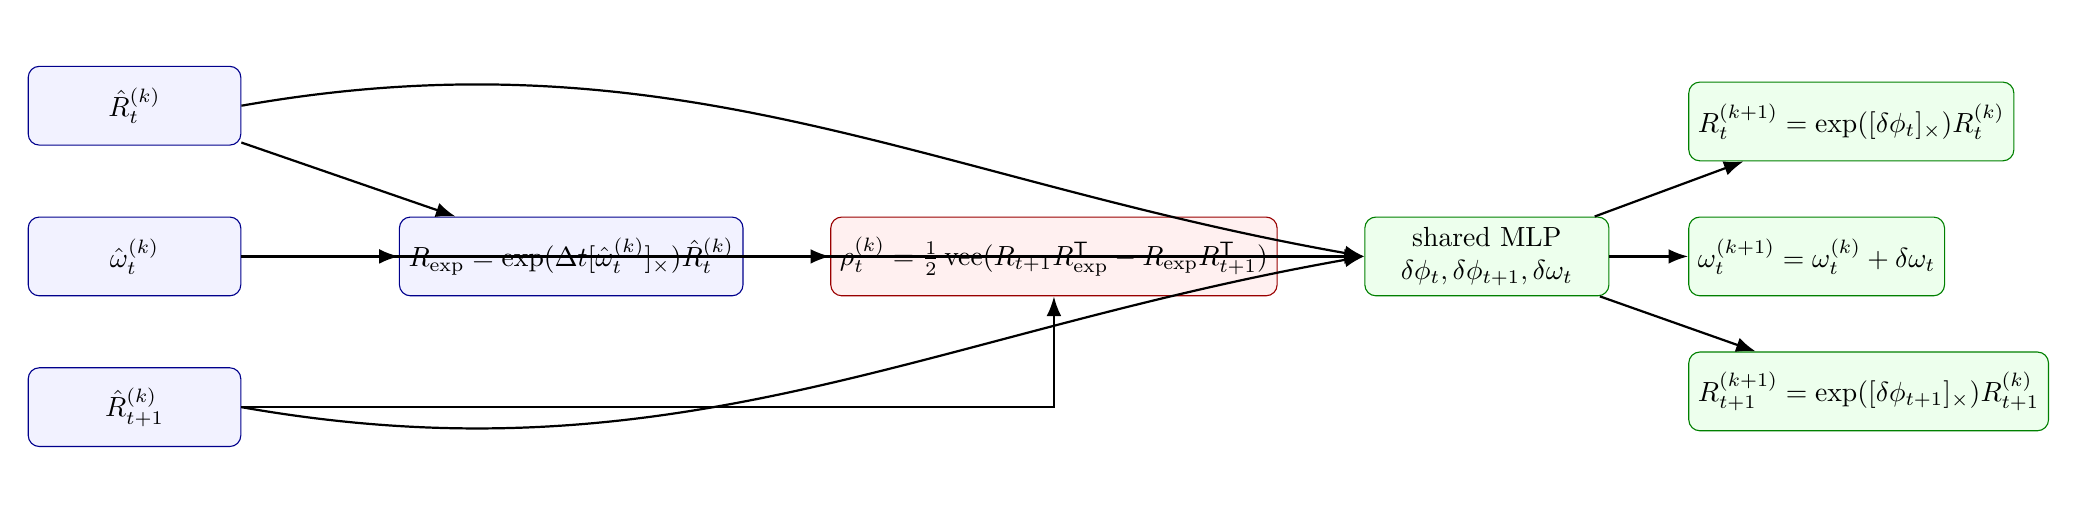
\begin{tikzpicture}[
  node distance=9mm and 11mm,
  box/.style={draw=blue!55!black, fill=blue!5, rounded corners, align=center, minimum height=10mm, minimum width=27mm},
  res/.style={draw=red!60!black, fill=red!6, rounded corners, align=center, minimum height=10mm, minimum width=30mm},
  upd/.style={draw=green!50!black, fill=green!7, rounded corners, align=center, minimum height=10mm, minimum width=31mm},
  arr/.style={-{Latex[length=2.5mm]}, thick}
]
\node[box] (r0) {$\hat R_t^{(k)}$};
\node[box, below=of r0] (w) {$\hat\omega_t^{(k)}$};
\node[box, below=of w] (r1) {$\hat R_{t+1}^{(k)}$};
\node[box, right=20mm of w] (exp) {$R_{\rm exp}=\exp(\Delta t[\hat\omega_t^{(k)}]_\times)\hat R_t^{(k)}$};
\node[res, right=of exp] (res) {$\rho_t^{(k)}=\frac12\operatorname{vee}(R_{t+1}R_{\rm exp}^{\mathsf T}-R_{\rm exp}R_{t+1}^{\mathsf T})$};
\node[upd, right=of res] (mlp) {shared MLP\\$\delta\phi_t,\delta\phi_{t+1},\delta\omega_t$};
\node[upd, above right=7mm and 10mm of mlp] (u0) {$R_t^{(k+1)}=\exp([\delta\phi_t]_\times)R_t^{(k)}$};
\node[upd, right=10mm of mlp] (uw) {$\omega_t^{(k+1)}=\omega_t^{(k)}+\delta\omega_t$};
\node[upd, below right=7mm and 10mm of mlp] (u1) {$R_{t+1}^{(k+1)}=\exp([\delta\phi_{t+1}]_\times)R_{t+1}^{(k)}$};
\draw[arr] (r0)--(exp);
\draw[arr] (w)--(exp);
\draw[arr] (r1)-|(res);
\draw[arr] (exp)--(res);
\draw[arr] (r0.east) to[out=10,in=170] (mlp.west);
\draw[arr] (w.east) to[out=0,in=180] (mlp.west);
\draw[arr] (r1.east) to[out=-10,in=190] (mlp.west);
\draw[arr] (res)--(mlp);
\draw[arr] (mlp)--(u0);
\draw[arr] (mlp)--(uw);
\draw[arr] (mlp)--(u1);
\end{tikzpicture}
}
\caption{One shared refinement iteration on $\SO(3)$. The final MLP layer is zero-initialised, so the corrector begins as the identity.}
\label{fig:corrector}
\end{figure}

At iteration $k$,
\begin{equation}
R_{\mathrm{exp},t+1}^{(k)}=\Exp(\Delta t[\hat\omega_t^{(k)}]_\times)\hat R_t^{(k)}.
\end{equation}
The relative error is
\begin{equation}
R_{\mathrm{rel},t}^{(k)}=\hat R_{t+1}^{(k)}(R_{\mathrm{exp},t+1}^{(k)})^\mathsf T.
\end{equation}
A bounded tangent-like residual is extracted from the antisymmetric part:
\begin{equation}
\vect\rho_t^{(k)}=\frac12\operatorname{vee}(R_{\mathrm{rel},t}^{(k)}-(R_{\mathrm{rel},t}^{(k)})^\mathsf T).
\end{equation}
This equals $\sin\theta\,\vect u$, approaching the Lie-algebra logarithm for small errors while remaining bounded near $\pi$. The shared corrector predicts $\delta\vect\phi_t$, $\delta\vect\phi_{t+1}$, and $\delta\vect\omega_t$, followed by
\begin{align}
R_t^{(k+1)}&=\Exp([\delta\vect\phi_t]_\times)R_t^{(k)},\\
R_{t+1}^{(k+1)}&=\Exp([\delta\vect\phi_{t+1}]_\times)R_{t+1}^{(k)},\\
\vect\omega_t^{(k+1)}&=\vect\omega_t^{(k)}+\delta\vect\omega_t.
\end{align}
When a frame receives proposals from its left and right intervals, matrix-column averages are reprojected through the continuous 6D map. This is an unrolled learned correction, not a guaranteed convergent projection.

\section{Training objectives}
The rotation-only objective is
\begin{equation}
\mathcal L=\lambda_R\mathcal L_R+\lambda_\omega\mathcal L_\omega+
\lambda_z\mathcal L_z+\lambda_{\rm kin}\mathcal L_{\rm kin}+
\lambda_{\rm rev}\mathcal L_{\rm rev}+\lambda_{\rm var}\mathcal L_{\rm var}.
\end{equation}

\paragraph{Orientation supervision.}
\begin{equation}
\mathcal L_R=\frac1{BT}\sum_{b,t}\theta(\hat R_{b,t},R_{b,t}^{\rm gt}).
\end{equation}

\paragraph{Angular-velocity supervision.}
\begin{equation}
\mathcal L_\omega=\operatorname{MSE}(\hat{\vect{\omega}}^{\rm norm},\vect{\omega}^{\rm norm,gt}).
\end{equation}

\paragraph{Bidirectional latent prediction.}
\begin{equation}
\mathcal L_z=\frac12\|\hat{\vect{z}}_{t+1}-\sg(\vect{z}_{t+1})\|^2+
\frac12\|\hat{\vect{z}}_t-\sg(\vect{z}_t)\|^2.
\end{equation}

\paragraph{Rotational kinematic consistency.}
\begin{equation}
\mathcal L_{\rm kin}=\theta\left(\hat{R}_{t+1},\Exp(\Delta t[\hat{\vect{\omega}}_t]_\times)\hat{R}_t\right)^2.
\end{equation}

\paragraph{Time reversal.}
\begin{equation}
\mathcal L_{\rm rev}=\|\hat{\vect{\omega}}_t^-+\hat{\vect{\omega}}_t^+\|^2.
\end{equation}

\paragraph{Anti-collapse variance floor.}
A penalty is applied when content or motion feature standard deviation falls below a fixed floor. This makes a constant predictive representation costly.

\begin{table}[H]
\centering
\caption{Rotation-only objective weights.}
\begin{tabularx}{\textwidth}{lclX}
\toprule
Term & Weight & Representative expression & Role\\
\midrule
Orientation & 1.0 & $\theta(\hat R,R^{\rm gt})$ & Anchors content to metric orientation.\\
Angular velocity & 1.0 & $\|\hat\omega^{\rm norm}-\omega^{\rm norm,gt}\|^2$ & Anchors motion to world-frame spin.\\
Latent prediction & 0.1 & $\|\hat z_{t+1}-z_{t+1}\|^2$ & Organises content predictively.\\
Rotational consistency & 0.01 & $\theta(\hat R_{t+1},\Exp(\Delta t\hat\omega_t)\hat R_t)^2$ & Couples orientation and angular velocity.\\
Time reversal & 0.1 & $\|\omega^-+\omega^+\|^2$ & Encourages odd motion under time reversal.\\
Variance floor & 0.01 & feature-variance penalty & Discourages collapse.\\
\bottomrule
\end{tabularx}
\end{table}

\section{Optimisation and evaluation protocol}
The network uses AdamW-style optimisation with learning rate $3\times10^{-4}$ and weight decay 0.05, bfloat16 mixed precision, gradient clipping at norm 1.0, deterministic training, and 100 configured epochs. The selected checkpoint is \texttt{best-051.ckpt}. The test evaluation contains 1,050 windows and 10,500 frame states. Interventions operate on 9,450 intervals.

Evaluation comprises four complementary tests:
\begin{enumerate}[leftmargin=*]
\item \textbf{Direct state accuracy}: geodesic orientation error and component-wise angular-velocity regression metrics.
\item \textbf{Trajectory inspection}: best, median, worst, and random context windows plotted over time.
\item \textbf{Temporal interventions}: sequence reversal, repeated final frame, and temporal shuffling.
\item \textbf{Frozen linear probes}: orientation and angular velocity decoded from named intermediate representations.
\end{enumerate}

\section{Rotation-only results}
\subsection{Orientation accuracy}
\begin{keyresult}
Across 10,500 evaluated frame states, the mean orientation error is \SI{0.5068}{\degree}, the median is \SI{0.4676}{\degree}, the 95th percentile is \SI{0.9705}{\degree}, and the maximum is \SI{3.5235}{\degree}.
\end{keyresult}

\begin{table}[H]
\centering
\caption{Aggregate intrinsic orientation error.}
\begin{tabular}{lr}
\toprule
Metric & Value\\
\midrule
Mean geodesic error & \SI{0.5068}{\degree}\\
Median geodesic error & \SI{0.4676}{\degree}\\
95th percentile & \SI{0.9705}{\degree}\\
Maximum & \SI{3.5235}{\degree}\\
Evaluated states & 10,500\\
\bottomrule
\end{tabular}
\end{table}

An orientation error below one degree for 95\% of frames is strong evidence that the marker-enabled rendering resolves rotational configuration accurately. The maximum error remains below four degrees, indicating that failures are bounded rather than catastrophic.

\subsection{Angular-velocity accuracy}
\begin{table}[H]
\centering
\caption{Component-wise angular-velocity results.}
\begin{tabular}{lrrrrr}
\toprule
Axis & RMSE [rad/s] & MAE [rad/s] & Bias [rad/s] & $R^2$ & Pearson\\
\midrule
$x$ & 0.3682 & 0.2702 & 0.0104 & 0.99958 & 0.99979\\
$y$ & 0.7487 & 0.3250 & -0.0344 & 0.99812 & 0.99907\\
$z$ & 0.4176 & 0.2951 & -0.1005 & 0.99943 & 0.99974\\
\bottomrule
\end{tabular}
\end{table}

\begin{figure}[H]
\centering
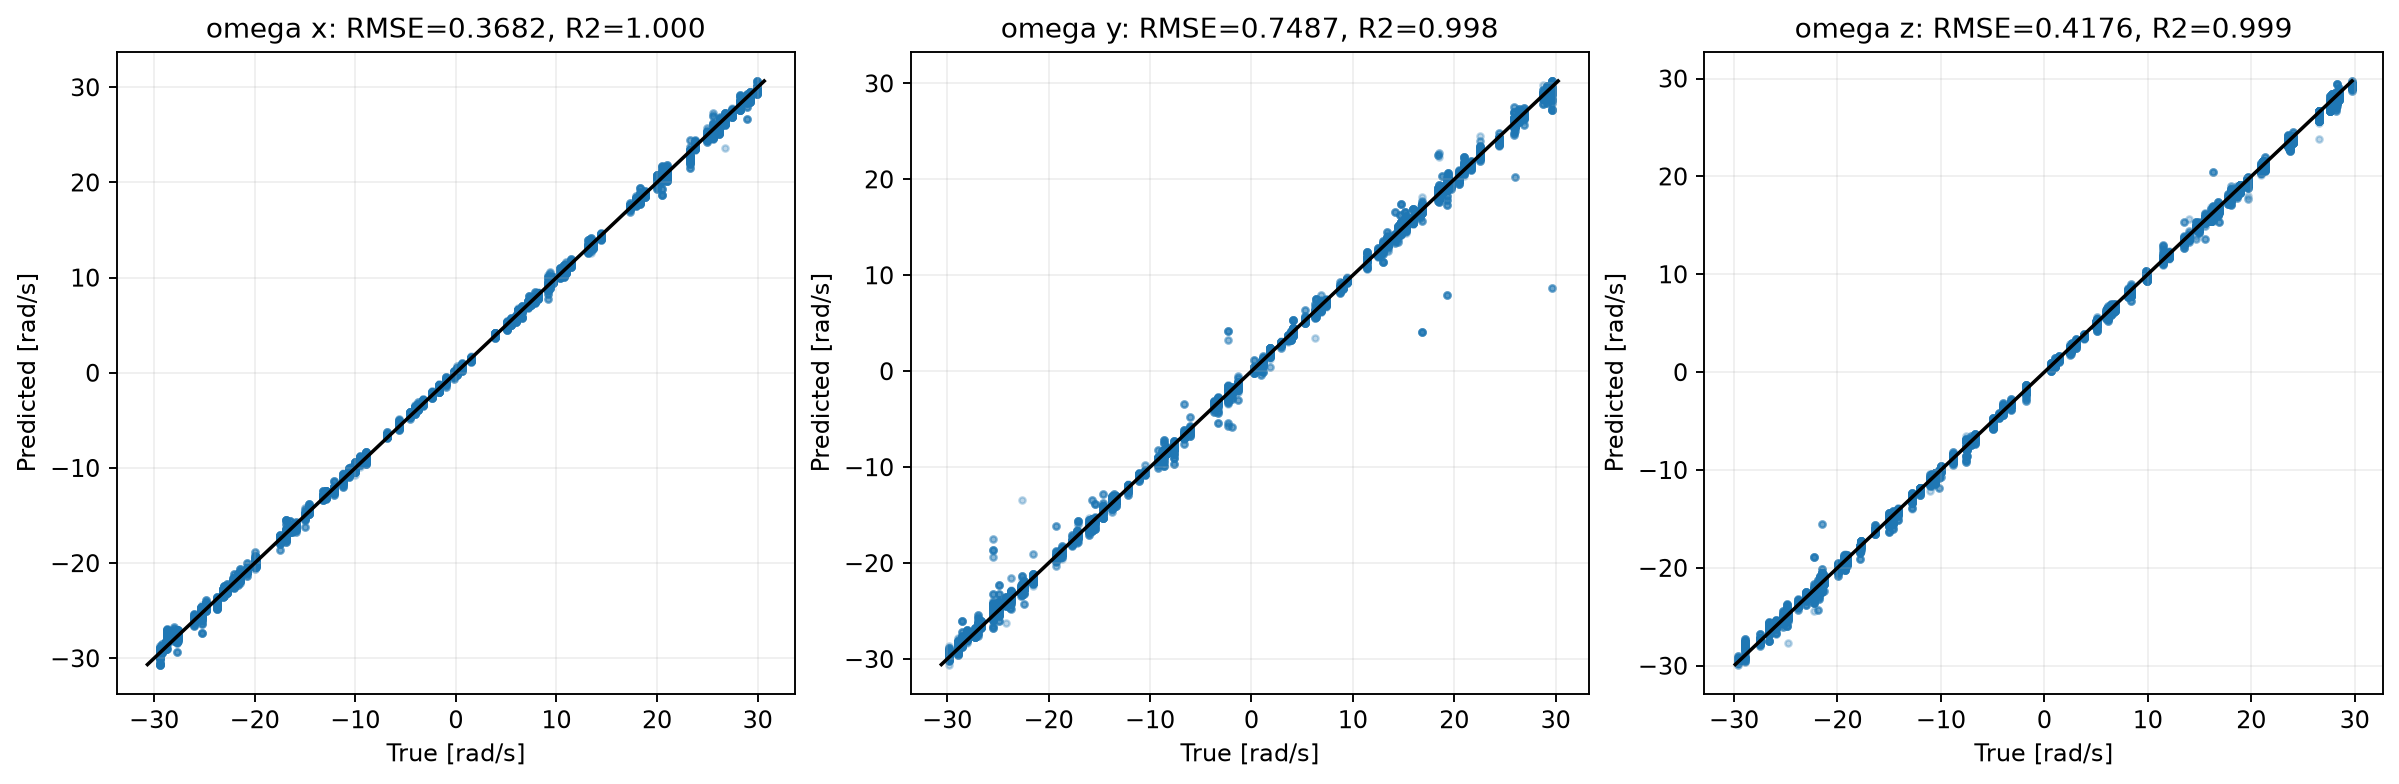
\includegraphics[width=.84\textwidth]{figures/angular_velocity_component_scatter.png}
\caption{Predicted versus true angular-velocity components. Points concentrate tightly around the identity line over the sampled range.}
\end{figure}

\begin{figure}[H]
\centering
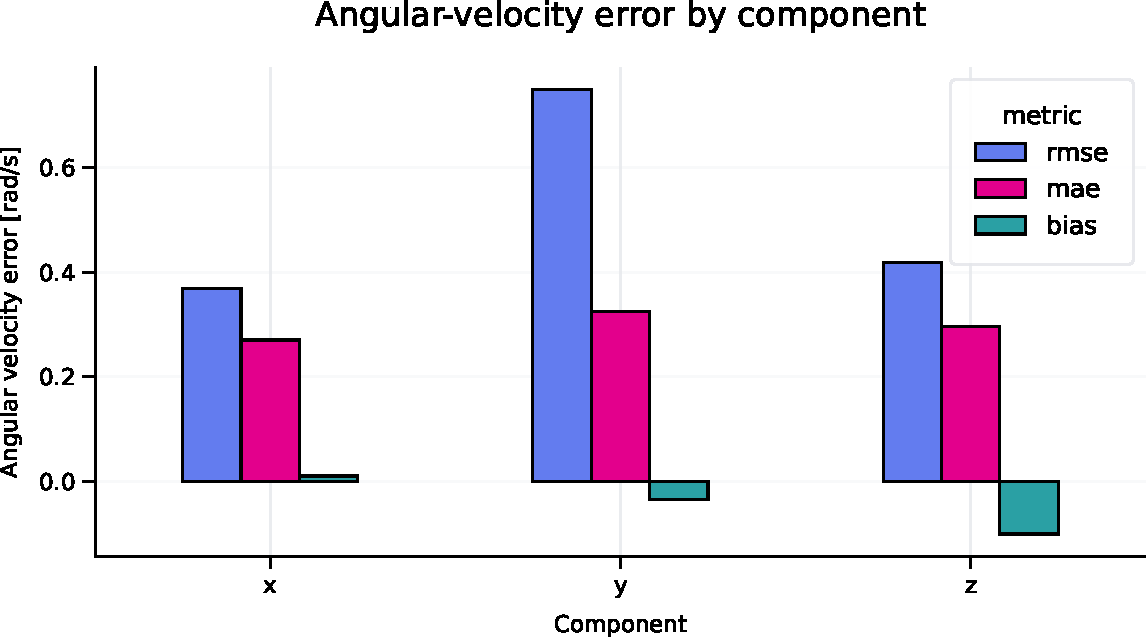
\includegraphics[width=.75\textwidth]{figures/omega_error_summary.pdf}
\caption{RMSE, MAE, and bias by angular-velocity component.}
\end{figure}

The $y$ component has the largest RMSE, but still explains 99.81\% of test variance. Error magnitude should be interpreted relative to the roughly \SI{29.3}{\radian\per\second} mean angular speed seen in the intervention set: the component RMSE values correspond to a small fraction of typical spin magnitude.

\subsection{Representative trajectories}
\begin{figure}[p]
\centering
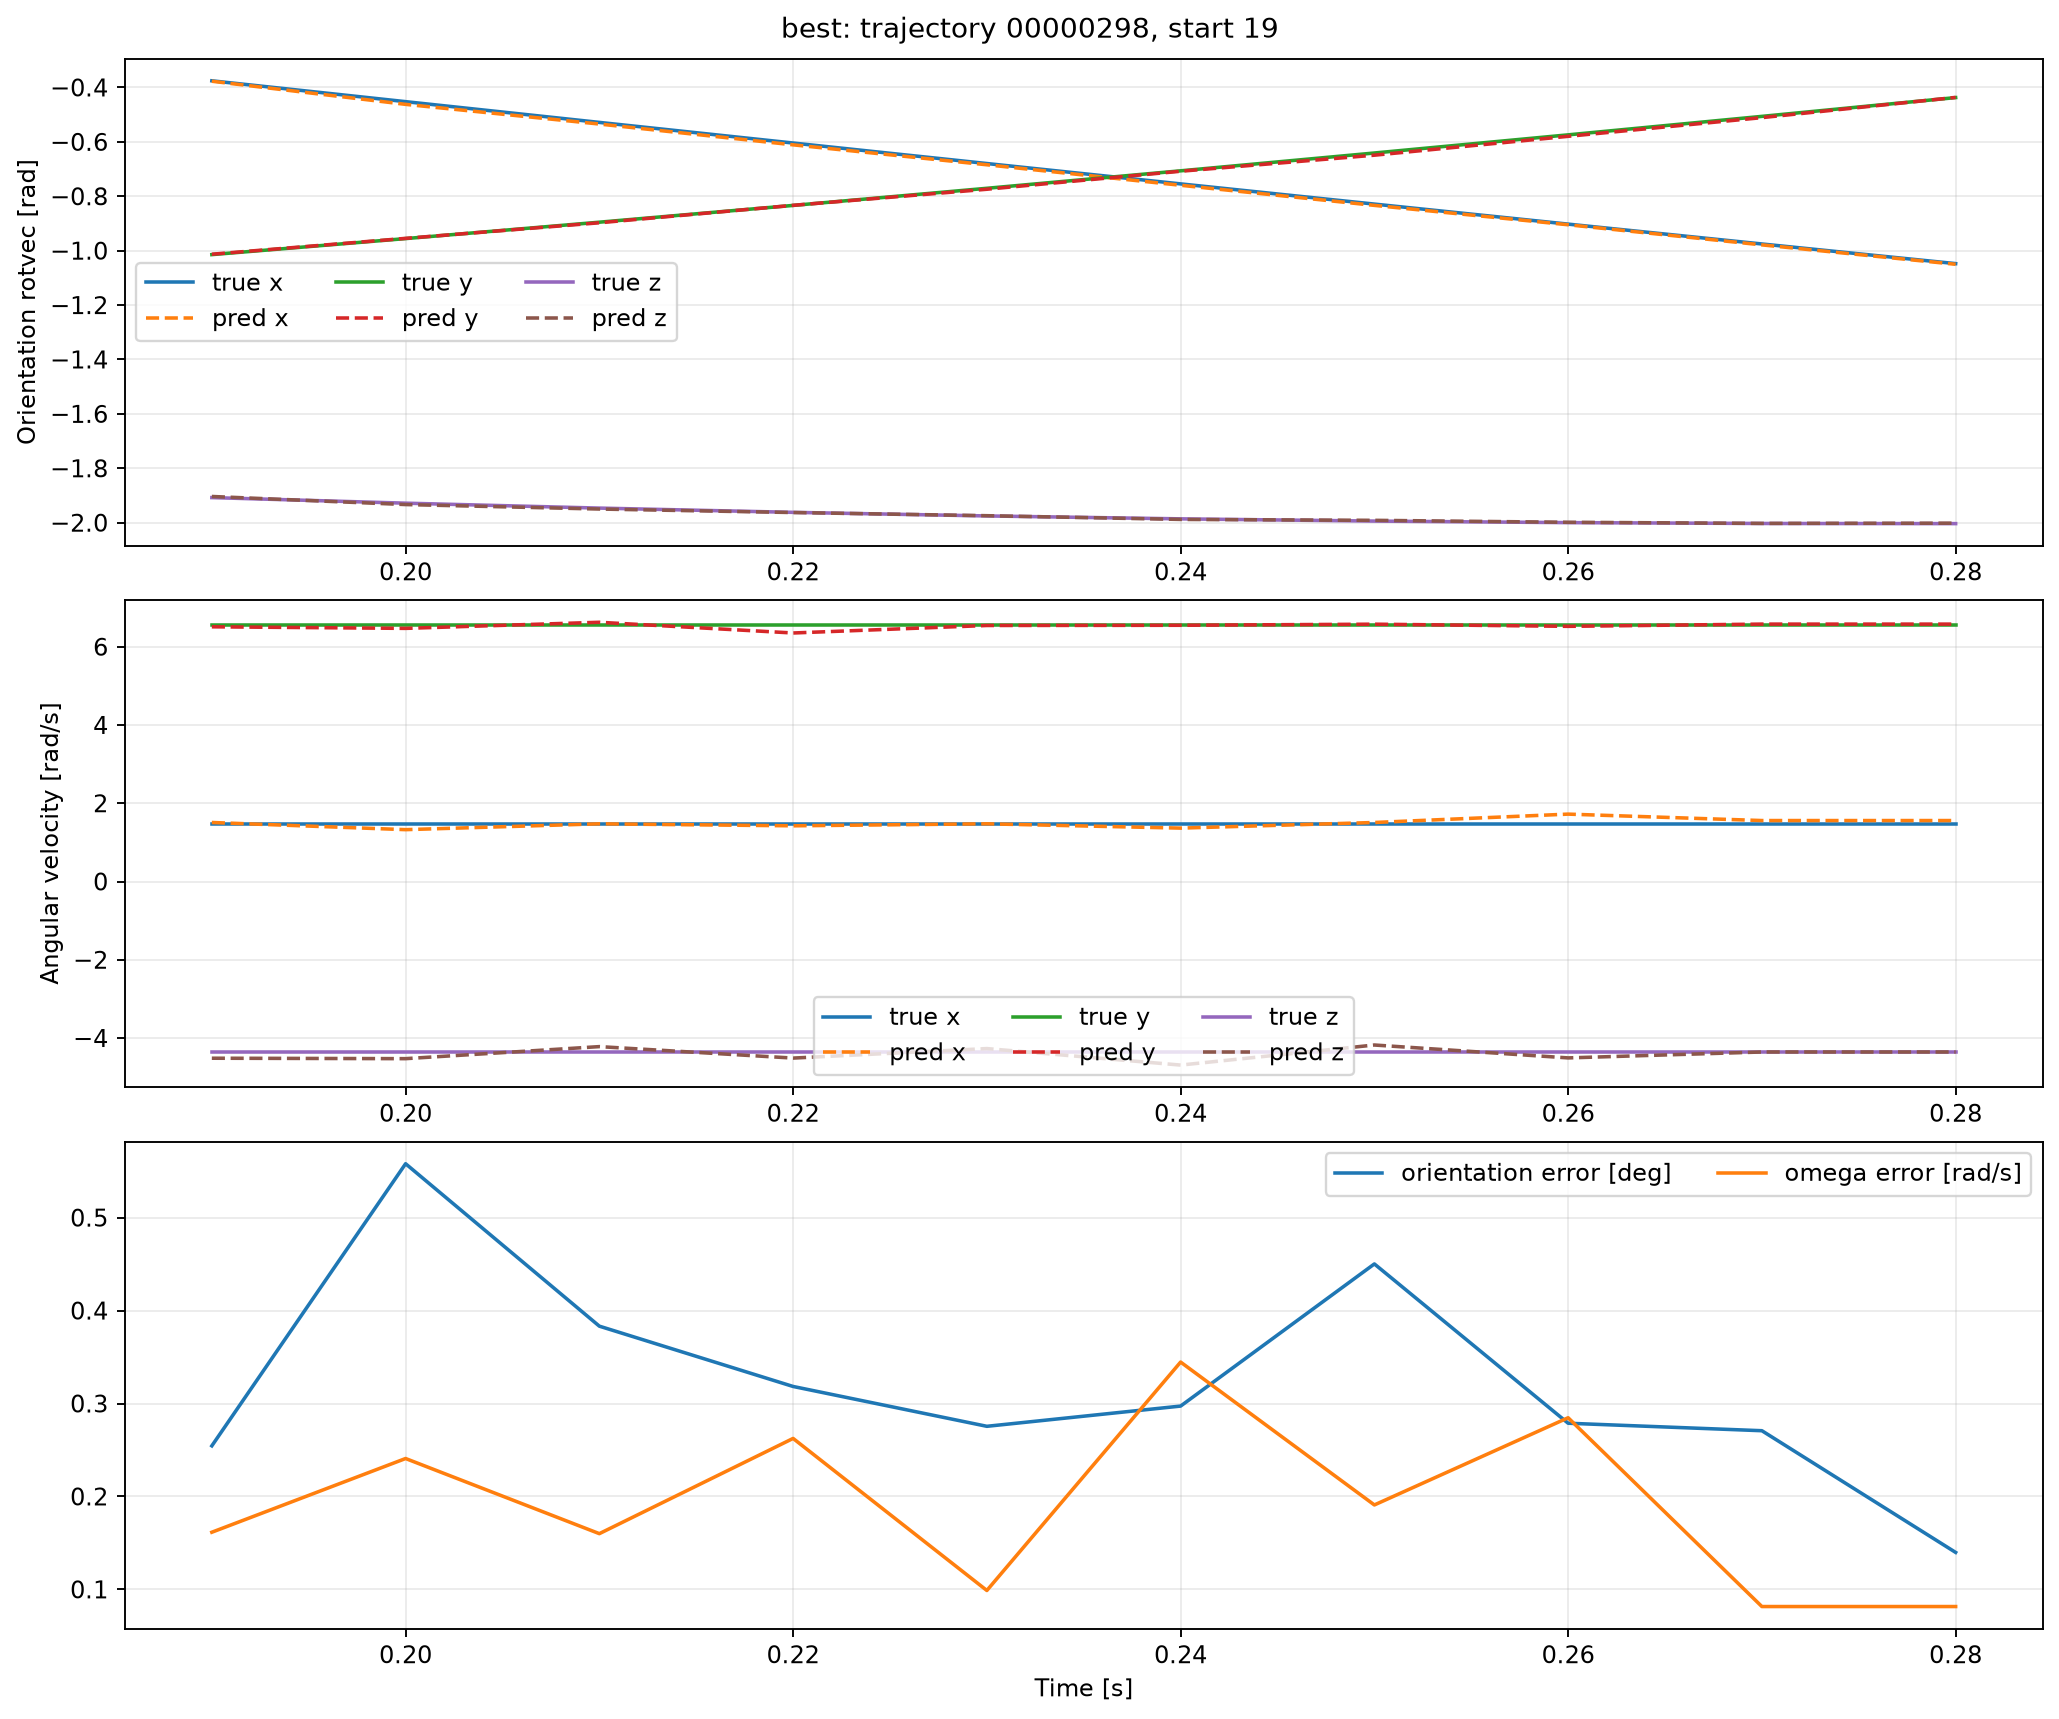
\includegraphics[width=.94\textwidth]{figures/best_00000298_000019.png}
\caption{Best evaluated window. Orientation and angular velocity remain close to ground truth throughout the context.}
\end{figure}
\begin{figure}[p]
\centering
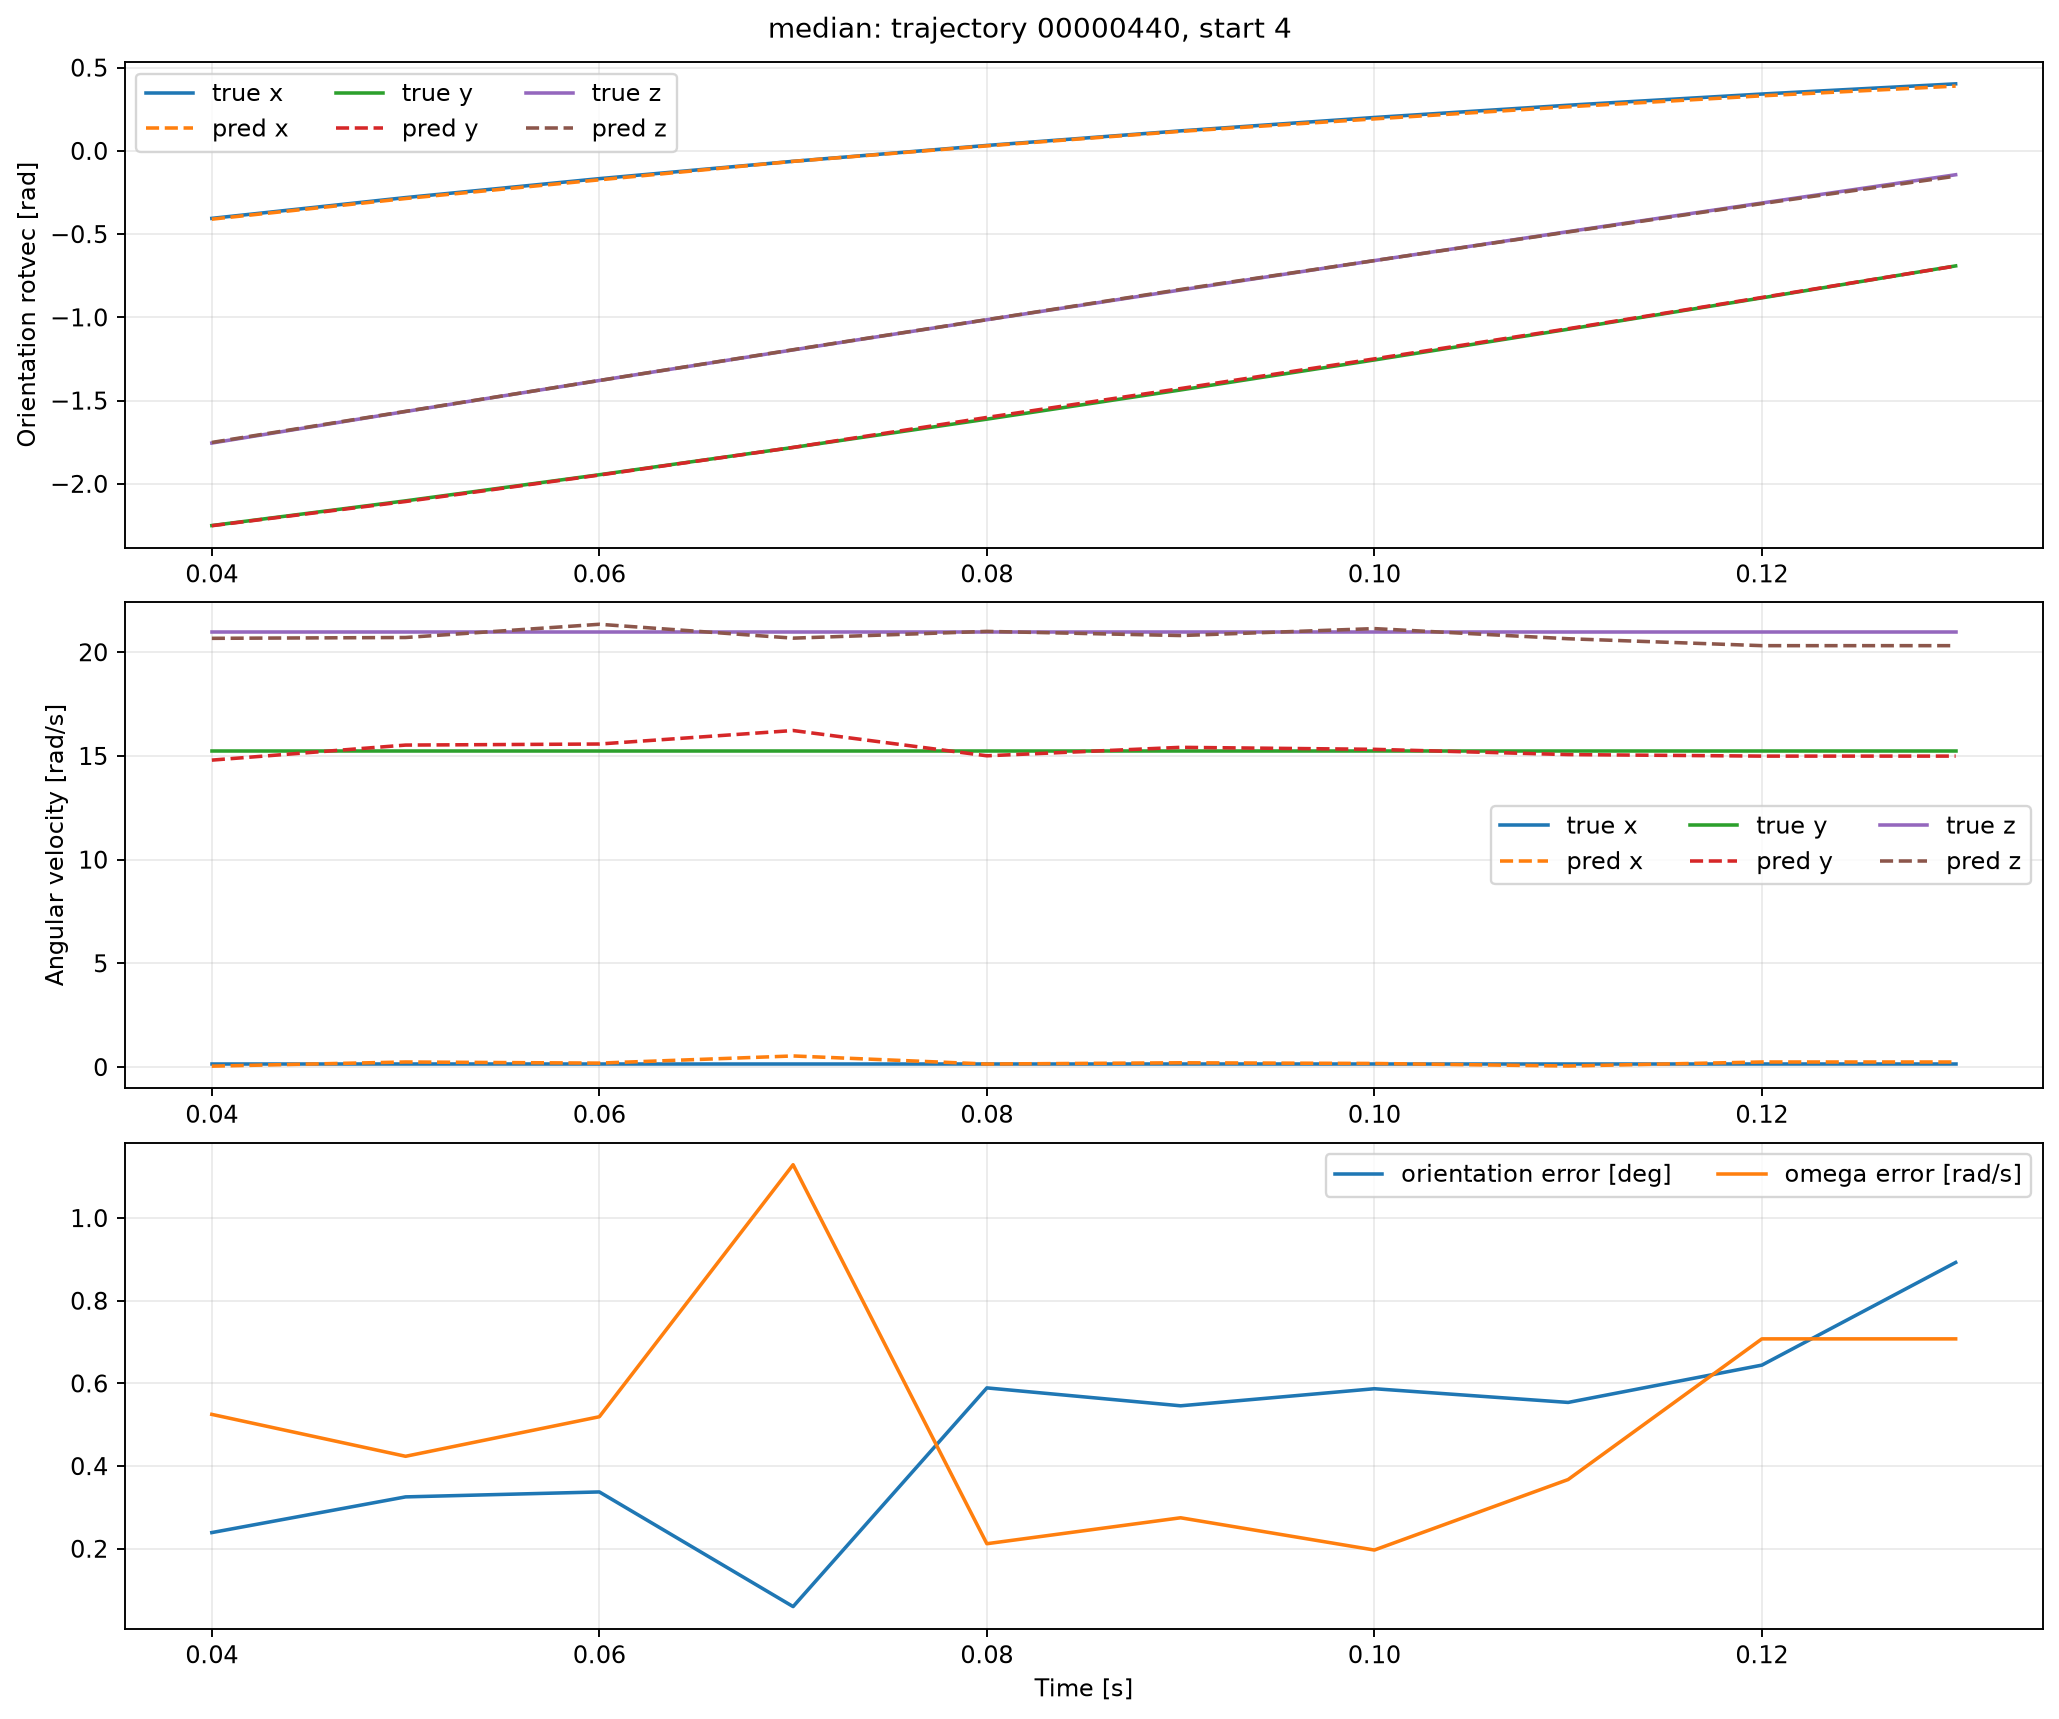
\includegraphics[width=.94\textwidth]{figures/median_00000440_000004.png}
\caption{Median evaluated window. The observer tracks a rapidly changing orientation while retaining nearly constant angular velocity.}
\end{figure}
\begin{figure}[p]
\centering
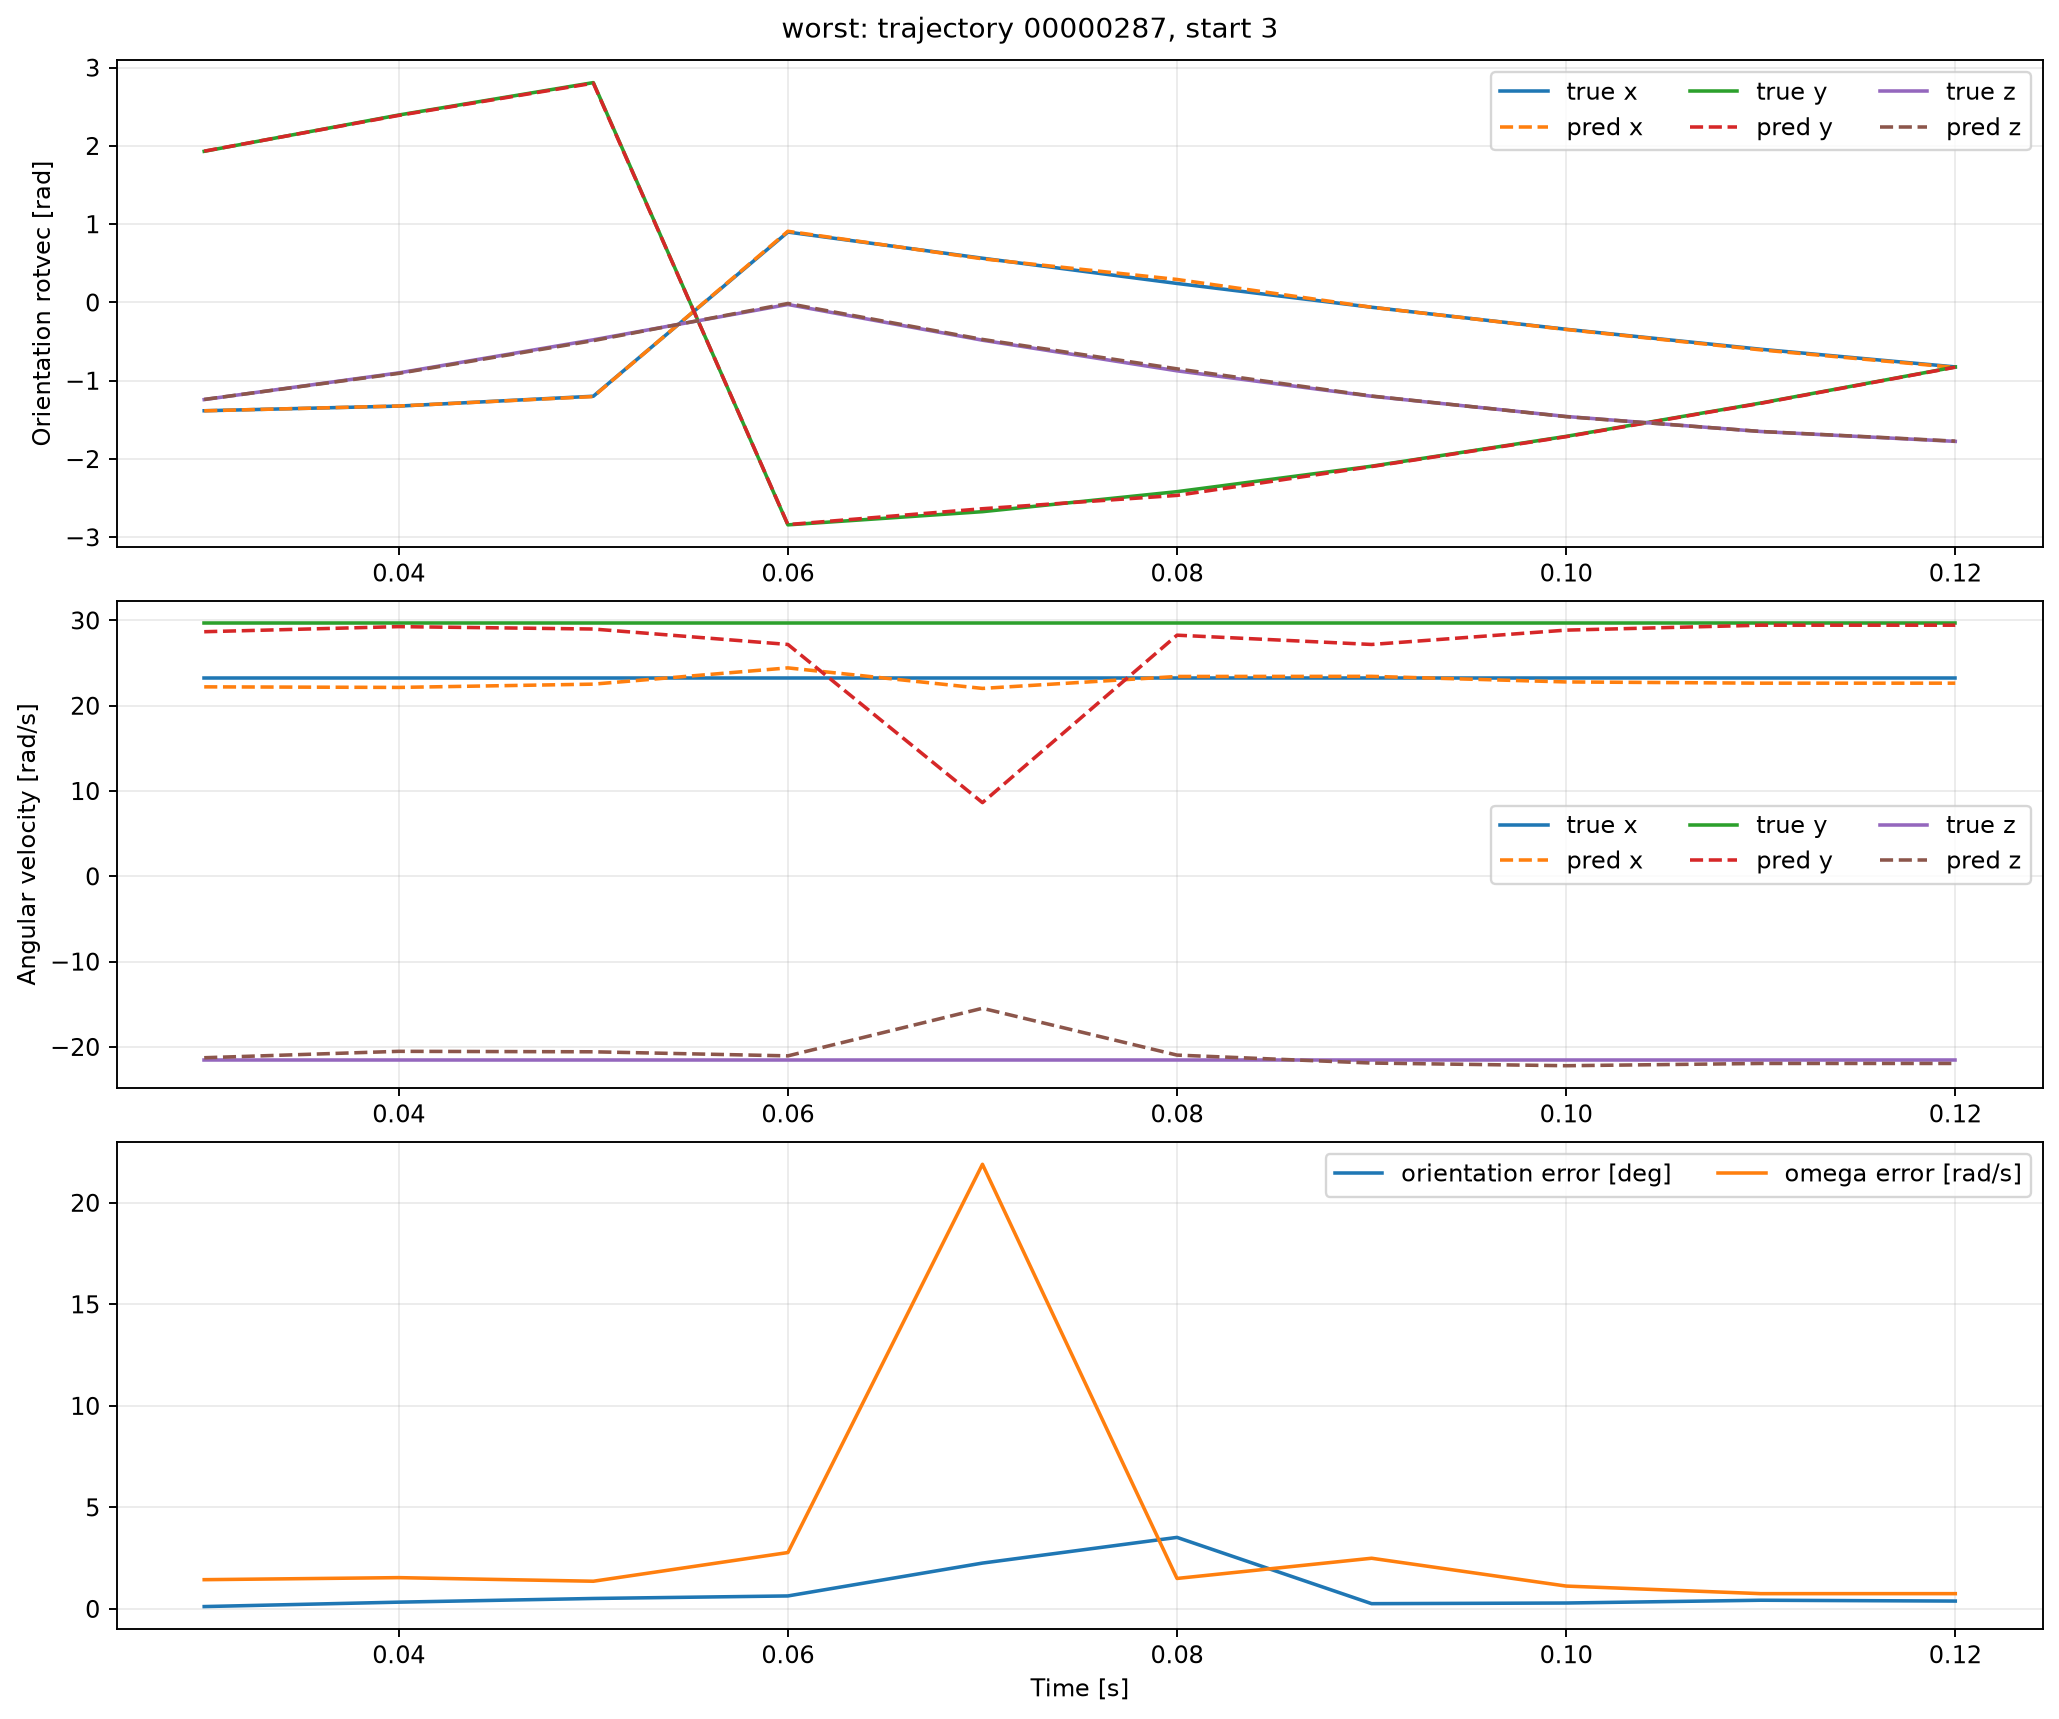
\includegraphics[width=.94\textwidth]{figures/worst_00000287_000003.png}
\caption{Worst evaluated window according to the combined trajectory score. Even this case remains bounded, with a maximum aggregate orientation error below \SI{3.53}{\degree}.}
\end{figure}
\FloatBarrier

\section{Temporal intervention analysis}
\begin{table}[H]
\centering
\caption{Intervention results over 9,450 intervals.}
\begin{tabular}{lrrrr}
\toprule
Input & Mean $\|\hat\omega\|$ & $\Delta$ from forward & Reversal error & Motion-latent change\\
 & [rad/s] & [rad/s] & [rad/s] & [latent units]\\
\midrule
Forward & 29.318 & 0.000 & 58.636 & 0.000\\
Reversed & 29.349 & 58.659 & 0.816 & 15.827\\
Repeated final frame & 0.382 & 29.336 & 29.305 & 12.258\\
Shuffled & 34.573 & 39.500 & 41.863 & 12.709\\
\bottomrule
\end{tabular}
\end{table}

\begin{figure}[H]
\centering
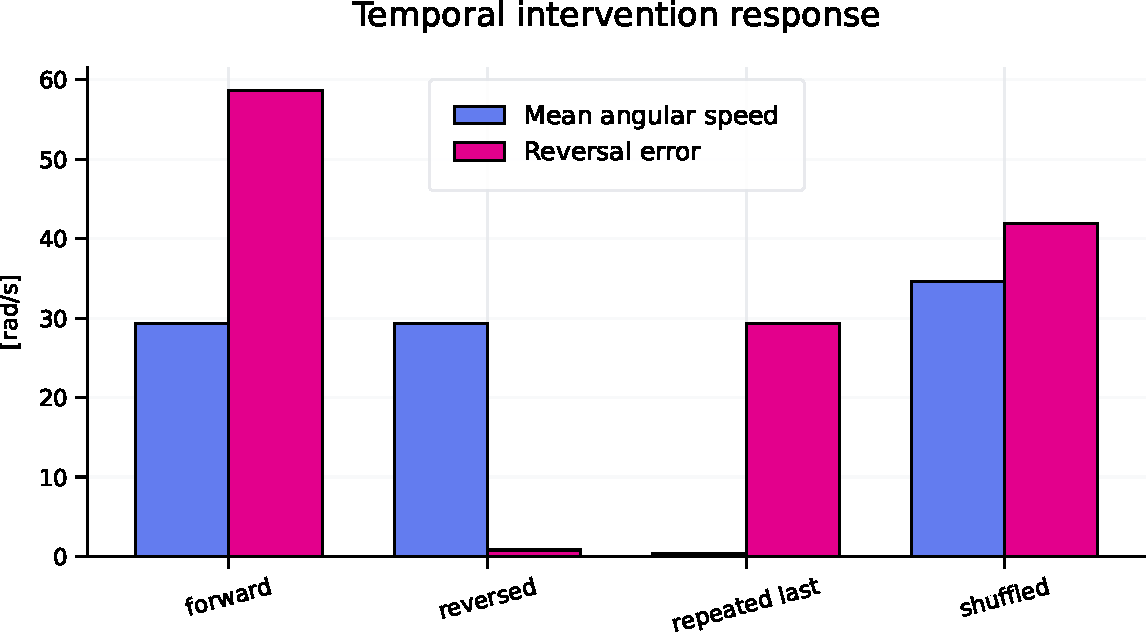
\includegraphics[width=.78\textwidth]{figures/interventions_summary.pdf}
\caption{Mean predicted angular speed and reversal error under temporal interventions.}
\end{figure}

\subsection{Reversal}
For perfect reversal, $\hat\omega_{\rm reversed}\approx-\hat\omega_{\rm forward}$. The observed mean difference between forward and reversed estimates is \SI{58.659}{\radian\per\second}, almost exactly twice the forward mean angular speed. The residual in the reversal relation is only \SI{0.816}{\radian\per\second}. The motion latent changes markedly, showing that the temporal direction is represented before the final state head.

\subsection{Repeated frames}
Using the final frame ten times reduces mean inferred angular speed from \SI{29.318}{\radian\per\second} to \SI{0.382}{\radian\per\second}, a reduction of approximately 98.7\%. Static orientation alone therefore does not determine predicted spin. This rejects a major shortcut hypothesis.

\subsection{Shuffling}
Temporal shuffling changes angular velocity by \SI{39.50}{\radian\per\second} on average and strongly changes the motion latent. The resulting mean speed rises to \SI{34.57}{\radian\per\second}; shuffled inputs are out of distribution, so the absolute value is not expected to be physically meaningful. The important conclusion is that order matters strongly.

\begin{caution}
Interventions are diagnostic rather than formal causal proofs. Reversed and shuffled sequences are outside the training distribution. Nevertheless, the simultaneous reversal of angular velocity, collapse under repeated frames, and strong motion-latent response provide compelling evidence that the observer uses temporal change.
\end{caution}

\section{Layer-wise representation analysis}
\begin{figure}[H]
\centering
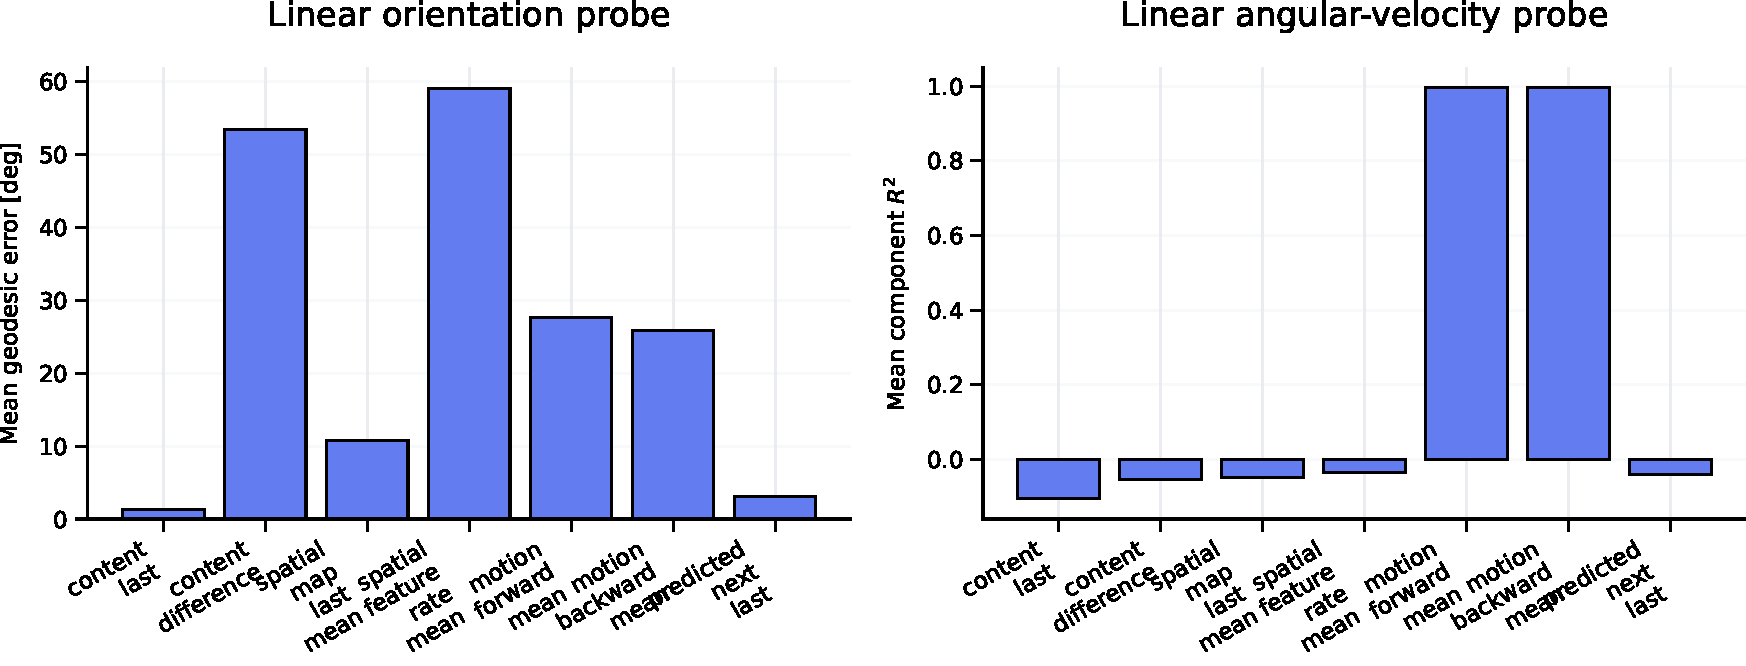
\includegraphics[width=.98\textwidth]{figures/probe_summary.pdf}
\caption{Frozen linear probes. Orientation is reported as mean geodesic error, where lower is better. Angular velocity is reported as mean component $R^2$, where higher is better.}
\end{figure}

\begin{landscape}
\begin{longtable}{p{.25\textwidth}rrp{.37\textwidth}}
\caption{Interpretation of layer-wise probes.}\label{tab:probes}\\
\toprule
Representation & Orientation mean [deg] & Angular velocity mean $R^2$ & Interpretation\\
\midrule
\endfirsthead
\toprule
Representation & Orientation mean [deg] & Angular velocity mean $R^2$ & Interpretation\\
\midrule
\endhead
Content last & 1.266 & -0.105 & Strong configuration information, no useful linear spin information.\\
Content difference & 53.431 & -0.055 & Raw compact-latent subtraction is not sufficient for rotational velocity in this model.\\
Spatial map last mean & 10.734 & -0.049 & Global feature pooling loses marker geometry and temporal direction.\\
Spatial feature-rate mean & 58.992 & -0.034 & Simple channel-wise averaging of feature rate destroys useful spatial motion organisation.\\
Motion forward mean & 27.664 & 0.9952 & Learned forward motion is highly linearly informative about angular velocity.\\
Motion backward mean & 25.809 & 0.9952 & Backward motion contains comparable reversed angular-velocity information.\\
Predicted next last & 3.077 & -0.040 & Predicted content retains substantial next-orientation information, not spin.\\
\bottomrule
\end{longtable}
\end{landscape}

\subsection{Content encodes orientation}
A linear decoder from the final content embedding obtains \SI{1.266}{\degree} mean geodesic error and \SI{3.554}{\degree} at the 95th percentile. This is less accurate than the trained nonlinear orientation head, but it demonstrates that orientation is organized in an approximately linearly accessible form.

\subsection{Motion encodes angular velocity}
The learned forward motion embedding gives mean component $R^2=0.9952$ for angular velocity. Per-axis values are 0.9972, 0.9918, and 0.9967. The backward embedding is nearly identical in quality. In contrast, the content embedding has negative angular-velocity $R^2$, as do raw content differences and globally pooled feature rates.

This result differs subtly from translation: for rotation, subtraction of compact content embeddings is not itself sufficient. Rotational changes of surface markers are highly nonlinear in image space and depend on current orientation. The learned spatial motion encoder successfully combines endpoint feature maps and normalized feature rate before pooling.

\begin{keyresult}
The intended factorisation is strongly supported: content carries orientation, while the learned directed motion representation carries angular velocity. The separation is not merely qualitative; it is visible through opposing probe performance and confirmed by temporal interventions.
\end{keyresult}

\section{Representation dimensionality and collapse checks}
\begin{figure}[H]
\centering
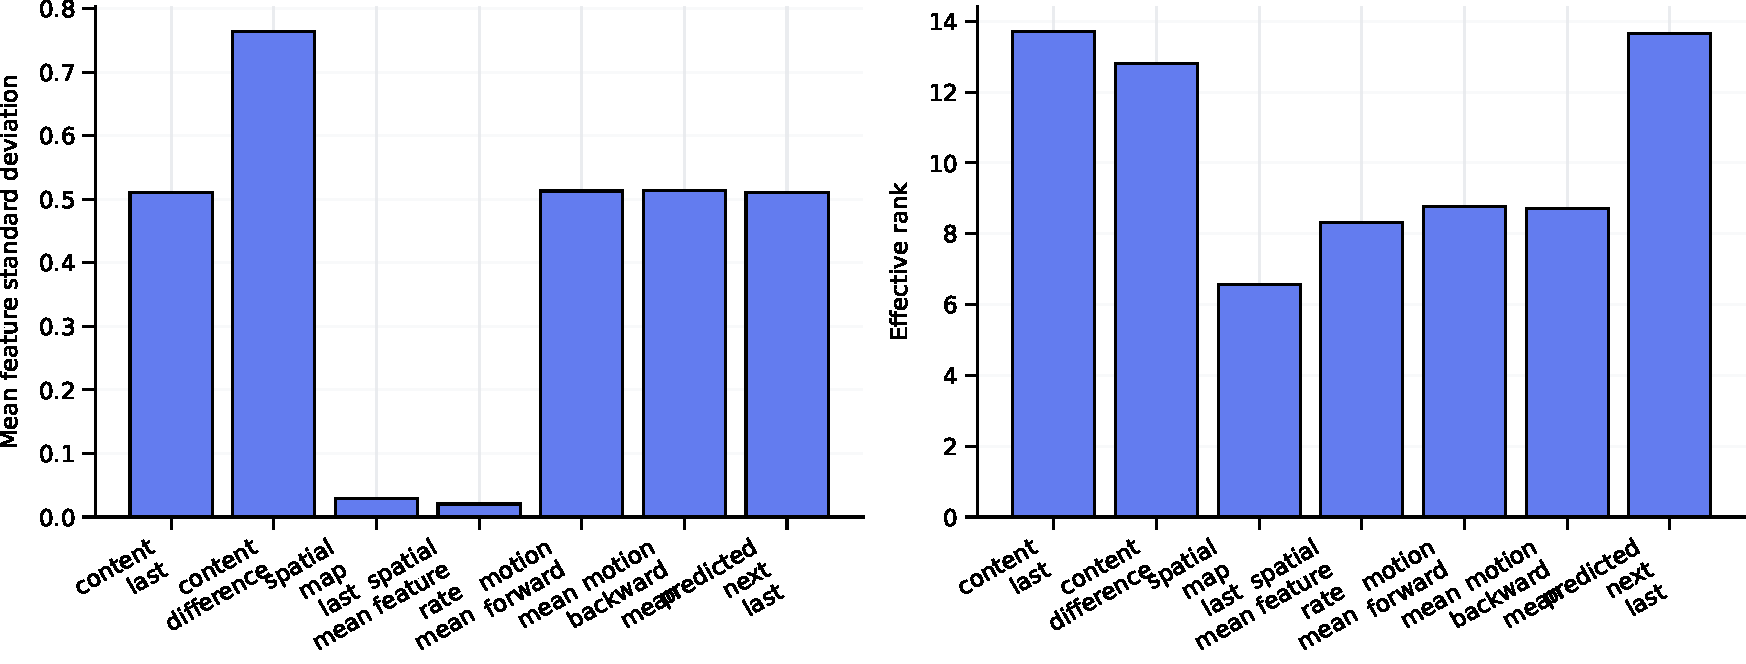
\includegraphics[width=.98\textwidth]{figures/representation_statistics.pdf}
\caption{Mean feature standard deviation and effective rank of the evaluated representations.}
\end{figure}

\begin{table}[H]
\centering
\caption{Representation statistics.}
\begin{tabular}{lrr}
\toprule
Representation & Mean feature std. & Effective rank\\
\midrule
Content last & 0.5108 & 13.725\\
Content difference & 0.7644 & 12.819\\
Spatial map last mean & 0.0295 & 6.562\\
Spatial feature-rate mean & 0.0204 & 8.315\\
Motion forward mean & 0.5129 & 8.766\\
Motion backward mean & 0.5134 & 8.710\\
Predicted next last & 0.5107 & 13.667\\
\bottomrule
\end{tabular}
\end{table}

No principal representation has collapsed to a constant. Content and motion have standard deviations near 0.51. The motion latent's effective rank near 8.7 is plausible for a low-dimensional rotational process with three orientation and three angular-velocity degrees of freedom plus visual nuisance coordinates. Effective rank is descriptive, not proof of a minimal physical coordinate system.

\section{Why the architecture succeeds}
The rotation-only results can be understood as the interaction of five design choices.

\begin{enumerate}[leftmargin=*]
\item \textbf{Marker-enabled rendering breaks spherical symmetry.} A perfectly uniform sphere provides no orientation observation. Surface markers create orientation-dependent image structure.
\item \textbf{Spatial differencing precedes global compression.} Marker motion remains localized in $16\times16$ feature maps rather than being averaged away.
\item \textbf{Content and motion have different jobs.} Orientation is decoded from content and spin from directed change, avoiding competition inside one undifferentiated temporal vector.
\item \textbf{Time reversal supplies a physically meaningful symmetry.} Reversed visual motion should reverse world angular velocity.
\item \textbf{The $SO(3)$ loss respects geometry.} Orientation is evaluated and coupled through relative rotation rather than through discontinuous Euler angles.
\end{enumerate}

\section{Threats to validity}
\subsection{Marker symmetry and identifiability}
The conclusions depend on the marker pattern uniquely identifying orientation over the sampled views. Symmetric or visually indistinguishable marker arrangements could create equivalent orientations. The current low geodesic error suggests that the used marker configuration is sufficiently informative in this controlled setting.

\subsection{Single camera and fixed centre}
The observer is trained for one fixed camera and one fixed centre. It may use camera-specific projection cues. Generalisation to new cameras, ball positions, radii, lighting, or marker layouts has not been established.

\subsection{Constant angular velocity}
The trajectory distribution contains constant angular velocity. Pairwise motion features may therefore rely on this regularity. Accelerating rotation, torque, drag, or collisions require a richer dynamics experiment.

\subsection{Probe interpretation}
A good linear probe shows decodability, not necessarily causal use. The intervention results strengthen the case for functional temporal use, but future latent interventions can test whether moving along an angular-velocity probe direction changes predicted rotation evolution.

\subsection{Corrector interpretation}
The iterative corrector is learned and unrolled for a fixed number of steps. It is not guaranteed to converge and should not be run for arbitrary extra iterations without an ablation.

\section{Recommended ablations}
\begin{enumerate}[leftmargin=*]
\item Compare refinement iterations $K=0$ and $K=1$ with identical data and seed.
\item Remove the reversal loss and repeat the intervention evaluation.
\item Remove latent prediction while retaining state supervision.
\item Replace the learned spatial motion encoder by pooled raw feature differences.
\item Train with fewer or smaller markers to map the observability boundary.
\item Vary context length and frame stride while supplying exact $\Delta t$.
\item Test held-out camera positions and small centre perturbations.
\item Train several seeds and compare motion representations using CKA or related similarity measures.
\end{enumerate}

\section{Relation to predictive coding and future world models}
The architecture shares a motivation with predictive coding: a useful internal state should explain temporal change rather than merely classify static appearance \citep{lotter2016prednet}. However, the current model predicts adjacent content embeddings, not pixels. This avoids allocating most loss weight to a static background while retaining a directly testable prediction target.

A future autonomous world model requires a transition that does not observe $F_{t+1}$. One route is
\begin{equation}
(\vect z_{t+1},\vect m_{t+1})=G(\vect z_t,\vect m_t),
\end{equation}
followed by state decoding. Another route uses the accurate decoded state and explicit rigid-body mechanics. A hybrid can use learned content and motion for perception, geometric state for physical rollout, and a latent residual for unmodeled effects.

The current rotation observer establishes a crucial precondition: orientation and angular velocity can be inferred accurately and represented separately from RGB. That result supports proceeding to combined translation and rotation, where content must encode both position and orientation and motion must encode both linear and angular velocity.

\section{Reproducibility checklist}
\begin{itemize}[leftmargin=*]
\item Fixed physical sphere parameters; only initial rotational state varies.
\item Fixed centre and zero linear velocity.
\item Fixed camera, marker layout, and renderer configuration.
\item Ten RGB frames at \SI{100}{Hz} with exact timestamps supplied to the model.
\item Trajectory-disjoint train, validation, and test partitioning.
\item Normalisation statistics computed on the training split and stored in checkpoints.
\item Evaluation checkpoint: \texttt{best-051.ckpt}.
\item Evaluation: 1,050 test windows, 10,500 frame states, and 9,450 interval interventions.
\item Aggregate metrics, interventions, probes, and representation statistics preserved as machine-readable CSV/JSON.
\item Old evaluation output cleared before writing a new run.
\end{itemize}

\section{Conclusion}
The rotation-only observer succeeds both numerically and representationally. Mean orientation error is approximately half a degree, angular-velocity $R^2$ exceeds 0.998 on every axis, and temporal interventions behave according to rotational physics. The content representation provides an accurate orientation coordinate, while the learned bidirectional motion representation provides an approximately linear angular-velocity coordinate. Repeated frames produce near-zero spin, reversed frames produce reversed spin, and shuffled frames strongly disrupt the motion estimate.

The most important conclusion is not a single RMSE value. It is the consistency of four independent observations: direct state accuracy, trajectory tracking, temporal interventions, and layer-wise probes. Together they show that the network has learned a meaningful separation between rotational configuration and rotational change. This validates the architecture as a strong visual state observer and provides a defensible foundation for combined six-degree-of-freedom state estimation and future autonomous latent dynamics.

\appendix
\section{Tensor-shape reference}
\begin{table}[H]
\centering
\begin{tabular}{lll}
\toprule
Quantity & Symbol & Shape\\
\midrule
RGB context & $I_{1:T}$ & $B\times10\times3\times256\times256$\\
Coordinate-augmented frame & $\tilde I_t$ & $B\times5\times256\times256$\\
Spatial features & $F_{1:T}$ & $B\times10\times128\times16\times16$\\
Soft-keypoint descriptor & $k_t$ & $B\times168$\\
Content embedding & $z_{1:T}$ & $B\times10\times256$\\
Feature rate & $\dot F_{1:T-1}$ & $B\times9\times128\times16\times16$\\
Forward motion & $m^+_{1:T-1}$ & $B\times9\times256$\\
Predicted rotation & $\hat R_{1:T}$ & $B\times10\times3\times3$\\
Interval angular velocity & $\hat\omega_{1:T-1}$ & $B\times9\times3$\\
Framewise angular velocity & $\hat\omega_{1:T}$ & $B\times10\times3$\\
\bottomrule
\end{tabular}
\end{table}

\section{Key numerical results}
\begin{itemize}[leftmargin=*]
\item Orientation mean/median/p95/max: 0.5068/0.4676/0.9705/3.5235 degrees.
\item Angular-velocity RMSE: 0.3682, 0.7487, and 0.4176 rad/s for $x,y,z$.
\item Angular-velocity $R^2$: 0.99958, 0.99812, and 0.99943.
\item Forward mean angular speed: 29.318 rad/s.
\item Reversed-sequence angular-speed reversal residual: 0.816 rad/s.
\item Repeated-frame mean angular speed: 0.382 rad/s.
\item Content-last orientation probe: 1.266 degrees mean error.
\item Motion-forward angular-velocity probe: mean $R^2=0.9952$.
\end{itemize}

\bibliographystyle{plainnat}
\bibliography{references}
\end{document}
